\documentclass{article}

\usepackage[margin=1in]{geometry}
\usepackage{amsmath}
\usepackage{amsfonts}
\usepackage{indentfirst}
\usepackage{bbm}
\usepackage{graphicx}
\graphicspath{ {../../Output/} }

\begin{document}

\section{Setup}
Suppose we have high-dimensional data $Z \in \mathbb{R}^{n \times q}$ with MDS embedding $X \in \mathbb{R}^{n \times p}$ for $p << q$. Given an out-of-sample point $w \in \mathbb{R}^q$, we want to compare various techniques for embedding $w$ into our $p$-dimensional embedding. We will consider the following techniques:
\begin{enumerate}
	\item Minimize absolute error in squared distances: $$\min_{y \in \mathbb{R}^q} \sum_{i=1}^n \left| d^2(w, z_i) - d^2(y, x_i) \right|$$
	\item Minimize squared error in distances: $$\min_{y \in \mathbb{R}^q} \sum_{i=1}^n \left( d(w, z_i) - d(y, x_i) \right)^2$$
	\item Trosset's MDS extension: $$\min_{y \in \mathbb{R}^q} \left\Vert 
	\begin{bmatrix}
	x_1^T \\
	\vdots \\
	x_n^2 \\
	y
	\end{bmatrix}
	\begin{bmatrix}
	x_1 & \cdots & x_n & y
	\end{bmatrix}
	 - \tau_w(A_2)\right\Vert^2$$
	 \item Trosset's approximate solution: $$y = (X^TX)^{-1}X^Tb$$
	 \item Bengio's MDS extension using $$\tilde{K}(a,b) = -\frac{1}{2}\left( d^2(a,b) - \frac{1}{2}\sum_{i=1}^n d^2(a, z_i) - \frac{1}{2}\sum_{i=1}^n d^2(b, z_i) + \frac{1}{n^2} \sum_{i=1}^n \sum_{j=1}^n d^2(z_i, z_j)\right)$$
\end{enumerate}

\noindent Note we include (1) and (2) because while (2) may seem more natural, CMDS minimizes a cost function of the same form as (1).

\section{Trosset Approx = Bengio (= PCA when using Euclidean distance)}
It turns out that Trosset's approximate solution and Bengio's solution are actually equal, regardless of the chosen dissimilarity measure. When the dissimilarity measure is Euclidean, both of these methods are equivalent to extending the PCA projection of the original data. To see why this is true, let's dissect the Bengio algorithm. Given the squared dissimilarity matrix $D_2$ of the original data, the algorithm uses the eigendecomposition of the double-centered matrix $$M = -\frac{1}{2}HD_2H.$$ The embedding is then given by $$y = \left(\frac{1}{\sqrt{\lambda_1}} v_1^T\tilde{w}, \hdots, \frac{1}{\sqrt{\lambda_q}} v_q^T\tilde{w}\right), \textrm{ where } \tilde{w} = 
\begin{bmatrix}
\tilde{K}(w, z_1) \\
\vdots \\
\tilde{K}(w, z_n)
\end{bmatrix}$$  and $(\lambda_i, v_i)$ are the eigenpairs of $M$. For Trosset's approximate solution, first note $X$ is the MDS embedding of $Z$, so $$X = \begin{bmatrix}
\vert & & \vert \\
v_1 & \cdots & v_q \\
\vert & & \vert
\end{bmatrix}
\begin{bmatrix}
\sqrt{\lambda_1} & & \\
& \ddots & \\
& & \sqrt{\lambda_q}
\end{bmatrix}.$$ Hence, $$y = (X^TX)^{-1}X^Tb = \left(\frac{1}{\sqrt{\lambda_1}} v_1^Tb, \hdots, \frac{1}{\sqrt{\lambda_q}} v_q^Tb\right).$$

\bigbreak It turns out that $\tilde{w} = b$ for all out-of-sample points $w \in \mathbb{R}^p$. This gives a clear interpretation of the matrix $$B = \tau_w(A_2) = \begin{bmatrix}
\tau_e(D_2) & b \\
b^T & \beta
\end{bmatrix}$$ for arbitrary squared dissimilarity matrices $A_2$. $B$ is the Gram matrix for points $z_1, \hdots, z_n, w$ using kernel $$\tilde{K}(a,b) = -\frac{1}{2}\left( d^2(a,b) - \frac{1}{n}\sum_{i=1}^n d^2(a, z_i) - \frac{1}{n}\sum_{i=1}^n d^2(b, z_i) + \frac{1}{n^2} \sum_{i=1}^n \sum_{j=1}^n d^2(z_i, z_j)\right).$$

\section{Min Cost Clustering}
When using absolute error in squared distances as the embedding cost function, we see a clustering of embedded points:

\begin{figure}[h]
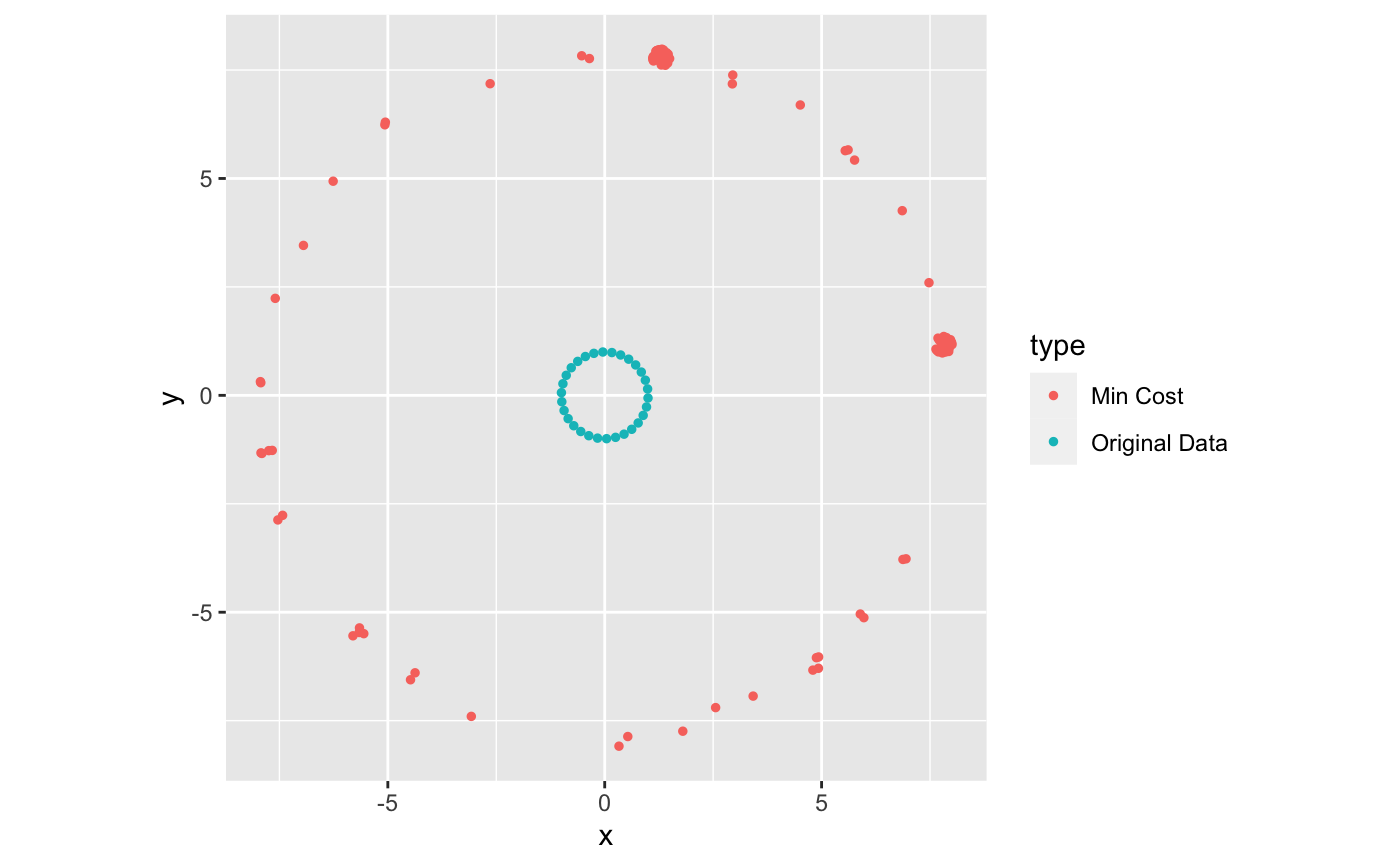
\includegraphics[scale=0.35]{Min cost clustering}
\centering
\end{figure}

\noindent This phenomenon is related to the $L_1$ regularization used in LASSO regression. It's well-known that the $L_1$ regularization term in LASSO regression forces some of the coefficient estimates to 0. The same is occurring here. The absolute cost function is embedding points so that $\left| d^2(w,z_i) - d^2(y, x_i) \right| = 0$ for some $i$. The points in each cluster all have $\left| d^2(w,z_i) - d^2(y, x_i) \right| = 0$ for the same $i$. For example in the configuration above, each point in the large cluster towards the top satisfies $\left| d^2(w,z_i) - d^2(y, x_i) \right| = 0$ for exactly $i = 2, 16$. Each point in the large cluster to the right satisfies $\left| d^2(w,z_i) - d^2(y, x_i) \right| = 0$ for exactly $i = 10, 26$.

\end{document}